\section{Reliablity-Related Bugs}

Software systems are getting more complex and new intricate bugs continue to
appear, causing billions of dollars in economic loss.  One notorious type of
software bugs is concurrency bugs.  These timing-related bugs manifest
non-deterministically, and hence are extremely difficult to detect, diagnose,
and fix.  A huge body of work exists in this space that focuses on ``local''
concurrency (LC) bugs in single-machine multi-threaded software, caused by
incorrect interleaving of memory accesses.

Unfortunately, the reliability of datacenter distributed systems is severely
threatened by non-deterministic concurrency bugs as well, which we refer as
{\em distributed concurrency (DC) bugs}.  
%
DC bugs cannot be directly tackled by LC bug techniques, and they cause fatal
implications such as operation failures, downtimes, data loss and
inconsistencies. 

\subsection{Distributed Concurrency (DC) Bugs}

Distributed systems execute many complicated distributed protocols on
hundreds/thousands of machines with no common clocks. Moreover, cloud systems
run on large clusters of unreliable commodity machines, an environment that
produces a growing number and frequency of failures, including ``surprising''
failures \cite{Birman+09-CloudAgenda, Henry09-AmazonFUD}.  This combination
makes distributed systems prone to DC bugs caused by non-deterministic timing
of distributed events such as message arrivals, node crashes, node reboots, and
timeouts. It is common to see complex failure-induced DC bugs such as the one
below.



\newcommand{\qbeg}{
\begin{quote}
%\begin{spacing}{0.9}
%\vminthree
}
\newcommand{\qend}{
%\vminten
%\end{spacing}
\end{quote}
}




\newcommand{\fev}[1]{\textcolor{Maroon}{\textit{#1}}}
\newcommand{\ev}[1]{\textcolor{gray}{\textbf{#1}}}


%\def \cbrk {\\}
\def \cbrk {}


\qbeg
{\small
{\bf ZooKeeper Bug \#335:}
\ev{(1)} Nodes A, B, C start with latest txid \#10 and elect
B as leader,
\ev{(2)} \fev{B crashes},
\ev{(3)} Leader election re-run; C becomes leader,
\ev{(4)} Client writes data; A and C commit new txid-value pair \{\#11:X\},
\ev{(5)} \fev{A crashes before} committing tx \#11,
\ev{(6)} C loses quorum,
\ev{(7)} \fev{C crashes},
\ev{(8)} \fev{A reboots} and \fev{B reboots},
\ev{(9)} A becomes leader,
\ev{(10)} Client updates data; A and B commit a new txid-value 
pair \{\#11:Y\},
\ev{(11)} \fev{C reboots after} A's new tx commit,
\ev{(12)} C synchronizes with A; C notifies A of \{\#11:X\},
\ev{(13)} A replies to C the ``diff'' starting 
with tx 12 (excluding tx \{\#11:Y\}!),
\ev{(14)} Violation: permanent data inconsistency as A and B
have \{\#11:Y\} and  C has \{\#11:X\}.
}
\qend



We look at 104 DC bugs from widely-deployed cloud-scale datacenter distributed
systems including Cassandra, Hadoop MapReduce, HBase, and ZooKeeper.
Statistically, Figure \ref{bars}a (\BFLT) shows that \pctFaultYes\ of
DC bugs must have at least one fault.  In more detail, Figure
\ref{bars}b-d (\BTO, \BCR, \BRB) shows the percentage of issues that
require timeouts, crashes and reboots respectively, including how many
instances of such faults must be there; the rest is other faults such
as disk errors (not shown).

\begin{figure}

\centerline{
\begin{tikzpicture}[font=\sffamily\footnotesize]
\begin{axis}[
xbar stacked,
y=0.8cm,
%width=5in,
width=\columnwidth,
%height=120pt,
xmin=0,
xmax=100,
bar width=12pt,  
%xmajorgrids=true,
%ylabel={Categorizations},
symbolic y coords={RB, CR, TO, FLT},
ytick=data,
yticklabels={{(d) RB, (c) CR, (b) TO, (a) FLT}},
every axis y label/.style={at={(ticklabel cs:0.5)},rotate=90,anchor=near ticklabel},
xticklabels={,,},
axis x line*=none,
x axis line style={opacity=0},
axis y line*=right
]
\addplot [fill=red!40] plot coordinates {(73.08,RB) (52.88,CR) (88.46,TO) (37.0,FLT)};
\addplot [fill=gray!40] plot coordinates {(20.19,RB) (34.62,CR) (11.54,TO) (63.0,FLT)};
\addplot [fill=pink!40] plot coordinates {(6.73,RB) (7.69,CR) (0,TO) (0,FLT)};
\addplot [fill=brown!40] plot coordinates {(0,RB) (4.81,CR) (0,TO) (0,FLT)};

\coordinate (rb0) at (36.54, -0.5);
\coordinate (rb1) at (83.175, -0.5);
\coordinate (rb2p) at (96.635, -0.5);
\coordinate (cr0) at (26.44, 99.5);
\coordinate (cr1) at (70.19, 99.5);
\coordinate (cr2) at (91.345, 99.5);
\coordinate (cr3p) at (97.595, 99.5);
\coordinate (toNo) at (44.23, 199.5);
\coordinate (toYes) at (94.23, 199.5);
\coordinate (fltNo) at (18.5, 299.5);
\coordinate (fltYes) at (68.5, 299.5);
\end{axis}

\node at (rb0) {0 (73\%)};
\node at (rb1) {1 (20\%)};
\node at (rb2p) {2+};
\node at (cr0) {0 (53\%)};
\node at (cr1) {1 (35\%)};
\node at (cr2) {2 (8\%)};
\node at (cr3p) {3+};
\node at (toNo) {No (88\%)};
\node at (toYes) {Yes (12\%)};
\node at (fltNo) {No (37\%)};
\node at (fltYes) {Yes (63\%)};

\end{tikzpicture}
%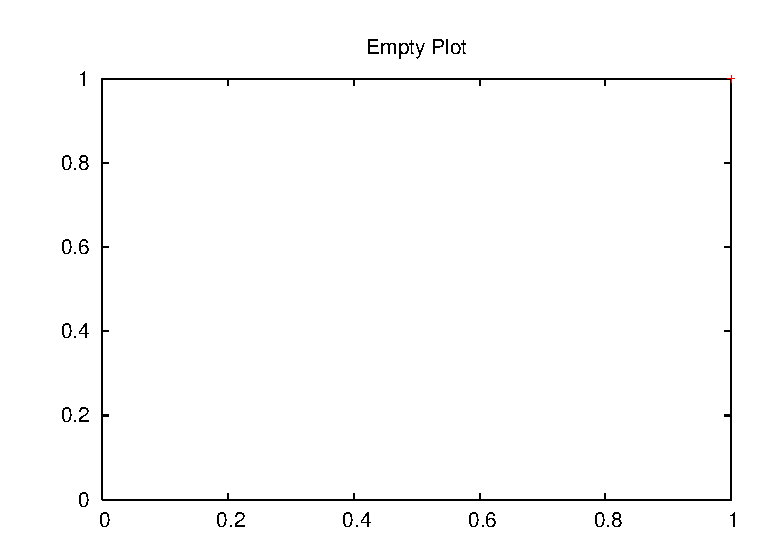
\includegraphics[width=1.8in]{F/empty.eps}
}
\vminten
\mycaption{bars}{Statistical overview of DC bugs}{}
% \vten

\end{figure}


%
\if 0
nodes (TSN), 
protocols (TSP), 
background (BR), 
triggering messages (TSM), 
local-message race (LM), 
timeout (TO),
crashes (CR),
reboots (RB),
errorMessage (EM),
reported (REP),  
implication (IMP),
control/data plane (CDP), 
\fi

